\documentclass[a4paper, 12pt, oneside]{scrartcl}
%\documentclass[a4paper, 12pt, oneside]{ncc}
\usepackage[warn]{mathtext}          % русские буквы в формулах, с предупреждением
\usepackage[T2A]{fontenc}            % внутренняя кодировка  TeX
\usepackage[utf8x]{inputenc}         % кодовая страница документа
\usepackage[english, russian]{babel} % локализация и переносы
\usepackage{indentfirst}   % русский стиль: отступ первого абзаца раздела
\usepackage{misccorr}      % точка в номерах заголовков
\usepackage{cmap}          % русский поиск в pdf
\usepackage{graphicx}      % Работа с графикой \includegraphics{}
\usepackage{psfrag}        % Замена тагов на eps картинкаx
\usepackage{caption2}      % Работа с подписями для фигур, таблиц и пр.
\usepackage{soul}          % Разряженный текст \so{} и подчеркивание \ul{}
\usepackage{soulutf8}      % Поддержка UTF8 в soul
\usepackage{fancyhdr}      % Для работы с колонтитулами
\usepackage{multirow}      % Аналог multicolumn для строк
\usepackage{amsmath, amssymb}
\usepackage{algorithm}
\usepackage{algpseudocode}
\usepackage{xcolor}
\usepackage{float}

	% Перевод данных об алгоритмах
	\renewcommand{\listalgorithmname}{Список алгоритмов}
	\floatname{algorithm}{Алгоритм}
	
	% Перевод команд псевдокода
	\algrenewcommand\algorithmicwhile{\textbf{До тех пока}}
	\algrenewcommand\algorithmicdo{\textbf{выполнять}}
	\algrenewcommand\algorithmicrepeat{\textbf{Повторять}}
	\algrenewcommand\algorithmicuntil{\textbf{Пока выполняется}}
	\algrenewcommand\algorithmicend{\textbf{Конец}}
	\algrenewcommand\algorithmicif{\textbf{Если}}
	\algrenewcommand\algorithmicelse{\textbf{иначе}}
	\algrenewcommand\algorithmicthen{\textbf{тогда}}
	\algrenewcommand\algorithmicfor{\textbf{Цикл}}
	\algrenewcommand\algorithmicforall{\textbf{Выполнить для всех}}
	\algrenewcommand\algorithmicfunction{\textbf{Функция}}
	\algrenewcommand\algorithmicprocedure{\textbf{Процедура}}
	\algrenewcommand\algorithmicloop{\textbf{Зациклить}}
	\algrenewcommand\algorithmicrequire{\textbf{Условия:}}
	\algrenewcommand\algorithmicensure{\textbf{Обеспечивающие условия:}}
	\algrenewcommand\algorithmicreturn{\textbf{Возвратить}}
	\algrenewtext{EndWhile}{\textbf{Конец цикла}}
	\algrenewtext{EndLoop}{\textbf{Конец зацикливания}}
	\algrenewtext{EndFor}{\textbf{Конец цикла}}
	\algrenewtext{EndFunction}{\textbf{Конец функции}}
	\algrenewtext{EndProcedure}{\textbf{Конец процедуры}}
	\algrenewtext{EndIf}{\textbf{Конец условия}}
	\algrenewtext{EndFor}{\textbf{Конец цикла}}
	\algrenewtext{BeginAlgorithm}{\textbf{Начало алгоритма}}
	\algrenewtext{EndAlgorithm}{\textbf{Конец алгоритма}}
	\algrenewtext{BeginBlock}{\textbf{Начало блока. }}
	\algrenewtext{EndBlock}{\textbf{Конец блока}}
	\algrenewtext{ElsIf}{\textbf{иначе если }}
	
\begin{document}

\section{Введение}

В этом отчёте производится сравнение двух алгоритмов поиска частых наборов бинарных данных - AD и DepthProject. На вход подается булева матрица $L = (a_{ij})$ размера $m \times n$, в которой элемент $a_{ij}$ равен 1, если в транзакции с номером $i$ значение порядка равно 1. Подается минимальная поддержка $s$ - целое число в диапазоне от 1 до m.

\section{Алгоритм AD}

\subsection{Описание}

Алгоритм AD строит частые наборы пошагово. Введём обозначения: R(L) - множество всех столбцов матрицы L, $S_1(L)$ - множество столбцов из R(L) с не менее чем s единицами, $e_1(R)$ и $e_2(R)$ - столбцы соответственно с наименьшим и наибольшим номерами в $R \subseteq R(L)$. Для набора $Q_t = {j_1, ..., j_t}$ обозначим $R_t$ - множество столбцов, номера которых больше $j_t$, $G_t$ - множество столбцов $h$ из $R_t$, которые в объединении с $Q_t$ дают совместимый набор.

Сначала строится первый частый набор $Q = {e_1(S_1(L))}$. Затем для каждого $Q = \{j_1, ..., j_r\} \neq \{e_2(S_1(L))\}$ строится следующий за ним набор $\Delta Q$ по следующим правилам:

1) $G_r \neq \varnothing$: $\Delta Q = Q \cup \{e_1(G_r)\}$;

2) $G_r = \varnothing$:

\qquad	a) $r = 1$: $\Delta Q = \{e_1(S_r)\}$;
	
\qquad	b) $r > 1$ и $G_{r-1} \neq \varnothing$: $\Delta Q = Q_{r-1} \cup {e_1(G_{r-1})}$;
	
\qquad	c) $r > 1$ и $G_{r-1} = \varnothing$: если $r = 2$, то $\Delta Q = \{e_1(R_r)\}$, иначе $\Delta Q = Q_{r-2} \cup \{e_1(R_{r-1})\}$;

Таким образом, алгоритм обходит дерево решений, вершины которого - частые наборы. Максимальные наборы находятся среди висячих вершин. В терминах алгоритма это значит, что если $G_t = \varnothing$, то $Q_t$ является либо максимальным частым набором, либо подмножеством ранее найденного максимального частого набора. Проверку на максимальность можно проводить как по ранее найденным наборам (тогда сложность алгоритма зависит от выхода задачи), так и по базе данных (модификация, предложенная Н. А. Драгуновым). Второй способ значительно быстрее.

Частый наборы выводятся в алфавитном порядке.

\subsection{Реализация}

Сначала строятся первый частый набор $Q[1] = \{e_1(R(L))\}$ и последний частый набор $L = \{e_2(R(L)\}$. Затем последовательно строятся наборы $Q[2], Q[3], ...$ из одной ветви дерева решений вплоть до первого максимального набора. После его нахождения начинает работать основной цикл, выход из которого осуществляется если очередной найденный набор равен $L$.

Используется процедура Обновить(T, Q), которая:

\quad 1) Зануляет строки матрицы T, дающие в пересечении со столбцами из Q нули.

\quad 2) Удаляет столбцы с номерами из Q.

Таким образом, первый совместимый столбец модифицированной матрицы есть первое частое расширение набора Q.

Ниже представлен псевдокод алгоритма AD:

\begin{algorithm}[H]
\caption{DepthProject}\label{alg:Examples}
\begin{algorithmic}[1]
\Procedure{AD}{$БазаДанных: T,\ Поддержка: s$}
	\State $Q = \varnothing$
	\State $L = ПоследнийЧастыйСтолбец(T, s)$
	\State $t = ПервыйЧастыйСтолбец(T, s)$
	\While{$t \neq \varnothing$}
		\State $Q = Q \cup \{e_1(G_r)\}$
		\Comment $r = |Q|$
		\State $Q\ -\ частый\ набор$
		\State $t = \{e_1(G_r)\}$
	\EndWhile
	\State $T' = T$
	\While{$Q \neq L$}
		\State $T' = Обновить(T', Q)$
		\State $t = ПервыйЧастыйСтолбец(T', s)$
		\If{$t \neq \varnothing$}
			\State $Q = Q \cup \{t\}$
		\Else
			\State $Q\ -\ частый\ набор$
			\State $Проверка\ Q\ на\ максимальность$
			\If{$|Q| = 1$}
				\State $Q = ПервыйЧастыйСтолбец(T', Q_1, s)$
			\Else
				\If{$|Q| = 2$}
					\State $Q = ПервыйЧастыйСтолбец(T', Q_1, s)$
				\Else
					\State $p = ПредпоследнийЭлемент(Q)$
					\State $T' = Обновить(T, Q_{r-2})$
					\State $t = ПервыйСовместимыйСтолбец(T', p, s)$
					\State $Q = Q \cup \{t\}$
				\EndIf
			\EndIf
		\EndIf
	\EndWhile
\EndProcedure
\end{algorithmic}
\end{algorithm}

\section{Алгоритм DepthProject}

\subsection{Пару слов о дереве решений}

В DepthProject производится рекурсивный обход дерева решения. Введём некоторые обозначения. Пусть имеется дерево решений $Д_L$:

1) Каждый узел соответствует частому набору. Корень дерева соответствует пустому набору элементов и обозначается $Null$.

2) Узел $P = \{i_1, ..., i_k\}$ имеет предка $Q = \{i_1, ..., i_{k-1}\}$.

Обозначим за $E(P)$ множество частых расширений узла $P$. Обозначим за $F(P)$ множество частых расширений родительского узла $Q$, номера которых превышают последний элемент в P. Справедливы вложения: $E(P) \subseteq F(P) \subset E(Q)$.

Алгоритм обходит это дерево решений и выводит наборы в алфавитном порядке. Древовидная структура позволяет на каждом шаге сужать область поиска частых расширений, рассматривая так называемых кандидатов. Преимущество такого подхода в том, что кандидаты ищутся за константное время по предыдущему узлу.

\subsection{Описание}

Вызывается процедура DepthFirst, на вход которой подаются узел N, база данных Т и маска B. При первом запуске N = Null, T - вся база данных (т.е. вся бинарная матрица), маска $B = (1, 1, ..., 1)$ - двоичный вектор длины $m$. В каноническом изложении процедура выглядит следующим образом:

\begin{algorithm}
\caption{DepthProject}\label{alg:Examples}
\begin{algorithmic}[1]
\Procedure{DepthFirst}{$Узел: N, БазаДанных: T, Маска: B$}
	\State $C = F(P)$
		\Comment{Множество кандидатов на частое расширение}
	\State $E = E(P)$
		\Comment{Множество частых расширений $E = \{i_1, ... , i_{|E|}\}$}
	\State $Положить\ N \cup i_r\ в\ узлы\ ДР$
	\State $B' = ПостроитьМаску(N, B, T)$
	\If {$Условие\ проекции$}
	    \State $T' = Проекция(T, E, N, B')$
	\Else
	    \State $T' = T$
	\EndIf
	\For{<r := 1 до |E|>}
		\State $DepthFirst(N \cup \{i_r\}, T', B')$
	\EndFor
\EndProcedure
\end{algorithmic}
\end{algorithm}

$F(P)$ - это номера столбцов из $E(Q)$, которые имеют номер, больший последнего номера в узле N. Здесь $Q$ - ближайший предок вершины $P$. Маска $B$ имеет 1 в $i-й$ позиции тогда и только тогда, когда все столбцы текущего узла имеют единицу в $i-й$ позиции. Проекция позволяет снизить время работы алгоритма. Вообще говоря, это аналог функции "Обновить" в реализации алгоритма AD с той лишь разницей, что строки и столбцы не зануляются, а удаляются. Уменьшая на каждом шаге базу данных T мы сужаем область поиска частых расширений $E(P)$. Также важно построить хороший метод поиска частых расширений.

\subsection{Реализация}

В текущей реализации DepthProject используется древовидная структура. Первым шагом находится множество кандидатов F(P) - эта операция производится быстро и сокращает дальнейший поиск частых расширений E(P). Маска готовится перед вызовом этих функций. Здесь маска - это логическое умножение столбцов текущего узла. Для её нахождения не обязательно перемножать все столбцы, достаточно на каждом шаге умножать текущую маску на последней столбец в узле. Итак, алгоритм примет вид:

\begin{algorithm}
\caption{DepthProject (реализованный)}\label{alg:Examples}
\begin{algorithmic}[1]
\Procedure{DepthFirst}{$Узел: N,\ Маска: B$}
	\State $B = ПостроитьМаску(N, B, T)$
	\State $C = E(N)$
	\State $E = E(N, T, B, C)$
	\For{<r := 1 до |E|>}
		\State $N \cup \{i_r\} \rightarrow \ множество\ частых\ наборов$
		\State $DepthFirst(N \cup \{i_r\}, T', B')$
	\EndFor
	\If $E = \varnothing$
		\If $N - максимальный\ набор$
			\State $N \rightarrow множество\ максимальных\ наборов$
		\EndIf
	\EndIf
\EndProcedure
\end{algorithmic}
\end{algorithm}

В этой реализации нет проекции, ведь можно обойтись без неё и даже получить выигрыш в скорости. В самом деле, зная маску и последний элемент в текущем узле мы легко найдём следующий совместимый столбец по исходной базе данных и потратим на всех подузлах столько же времени, сколько занимает одна проекция. \color{red} Возможно, есть способ сделать проекцию быстрее поиска с маской, но преимущество в скорости должно быть достаточно большим, поскольку сам факт рекурсивной передачи столь большого массива данных занимает определённое время. На практике одна лишь передача базы данных без последующей проекции увеличивает время работы алгоритма в два раза. Так или иначе, ни на количество шагов, ни на сложность шага это не влияет. Проекция - програмистское ухищрение авторов алгоритма, которое позволило им получить прирост в скорости. В моей реализации преимущество в скорости даёт маска и знание последнего элемента текущего узла.

\color{black}

\section{Сравнение двух алгоритмов}

При реализации алгоритмов использовалась одна и та же  модель бинарной матрицы. В обоих алгоритмах маска - это бинарный вектор bitset (C++ 11 версии и выше).

На вход подаётся бинарная матрица, m - кол-во строк (транзакций), n - кол-во столбцов (элементов). Минимальная поддержка s = 0.1.

\begin{table}[H]
\begin{tabular}{|c|c|c|c|}
\hline
                  & \textbf{n = 10}                                                & \textbf{n = 20}                                                 & \textbf{n = 30}                                                   \\ \hline
\textbf{m = 10}   & \begin{tabular}[c]{@{}c@{}}183, 5\\ 0.73\\ 2.56\end{tabular}   & \begin{tabular}[c]{@{}c@{}}49557, 10\\ 49\\ 52\end{tabular}     & \begin{tabular}[c]{@{}c@{}}1029918, 10\\ 1064\\ 4250\end{tabular} \\ \hline
\textbf{m = 100}  & \begin{tabular}[c]{@{}c@{}}169, 76\\ 0.89\\ 1.52\end{tabular}  & \begin{tabular}[c]{@{}c@{}}1560, 785\\ 3.39\\ 6.52\end{tabular} & \begin{tabular}[c]{@{}c@{}}9165, 4962\\ 16.1\\ 17.3\end{tabular}  \\ \hline
\textbf{m = 1000} & \begin{tabular}[c]{@{}c@{}}172, 117\\ 1.34\\ 1.87\end{tabular} & \begin{tabular}[c]{@{}c@{}}1350, 1136\\ 6.2\\ 8.6\end{tabular}  & \begin{tabular}[c]{@{}c@{}}4518, 4053\\ 23.3\\ 33.9\end{tabular}  \\ \hline
\end{tabular}
\end{table}

В первой строке - кол-во частых наборов и кол-во макс. частых наборов. Во второй строке время работы AD в миллисекундах, в третьей - время работы DepthProject. Результаты были усреднены по 20 запускам.

Ниже приведена аналогичная таблица для минимальной поддержки s = 0.3.

\begin{table}[H]
\begin{tabular}{|c|c|c|c|}
\hline
                  & \textbf{n = 10}                                        & \textbf{n = 20}                                                & \textbf{n = 30}                                                \\ \hline
\textbf{m = 10}   & \begin{tabular}[c]{@{}c@{}}64, 10\\ 0.184\\ 0.398\end{tabular} & \begin{tabular}[c]{@{}c@{}}573, 30\\ 1.62\\ 1.73\end{tabular}  & \begin{tabular}[c]{@{}c@{}}1225, 43\\ 2.6\\ 11.2\end{tabular}  \\ \hline
\textbf{m = 100}  & \begin{tabular}[c]{@{}c@{}}16, 10\\ 0.084\\ 0.2\end{tabular}   & \begin{tabular}[c]{@{}c@{}}50, 34\\ 0.383\\ 0.216\end{tabular} & \begin{tabular}[c]{@{}c@{}}110, 86\\ 0.924\\ 1.26\end{tabular} \\ \hline
\textbf{m = 1000} & \begin{tabular}[c]{@{}c@{}}10, 10\\ 0.154\\ 0.222\end{tabular} & \begin{tabular}[c]{@{}c@{}}20, 20\\ 0.533\\ 0.693\end{tabular} & \begin{tabular}[c]{@{}c@{}}30, 30\\ 0.817\\ 1.043\end{tabular} \\ \hline
\end{tabular}
\end{table}

Алгоритм AD немного быстрее, особенно в тех моментах, когда количество всех частых наборов много больше максимальных частых наборов. Нетрудно догадаться, что в этом случае дерево решений имеет большую глубину. Следовательно, рекурсивный вызов процедуры DepthProject имеет большую вложенность, а передача объектов в процедуру нагружает процессор. В этом и заключается преимущество последовательного подхода.

\newpage

Изобразим на графике зависимость времени работы двух алгоритмов от количества столбцов при фиксированном количестве строк.

\begin{figure}[H]
\center{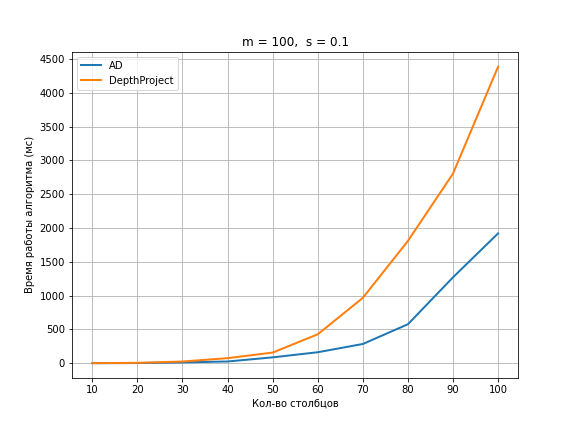
\includegraphics[scale=0.5]{r3p1.png}}
\caption{Зависимость времени работы от кол-ва столбцов}
\label{fig:image}
\end{figure}

Как видим, скорости счёта двух алгоритмов отличаются в константное число раз. Изобразим на графике отношение времени работы алгоритмов:

\begin{figure}[H]
\center{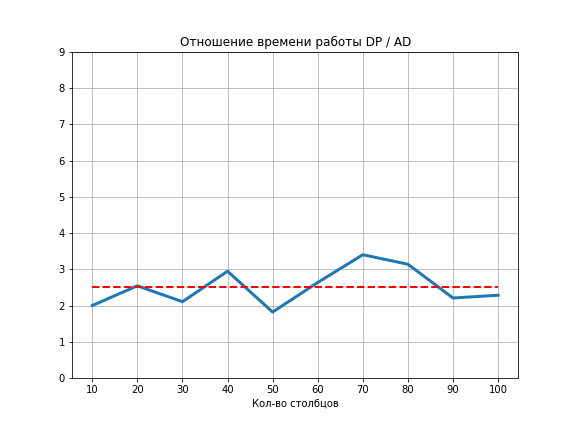
\includegraphics[scale=0.5]{r3p2.png}}
\caption{Отношение времени работы DepthProject и AD}
\label{fig:image}
\end{figure}

В среднем скорость счёта отличается в 2.5 раза. Это подтверждает тот факт, что алгоритмы совершают одинаковое число шагов. Сложность шага в DepthProject чуть больше, но это связано исключительно с реализацией.

\newpage

Теперь изобразим на графике зависимость времени работы двух алгоритмов от количества строк при фиксированном количестве столбцов. Положим $n = 20$, $s = 0.1$:

\begin{figure}[H]
\center{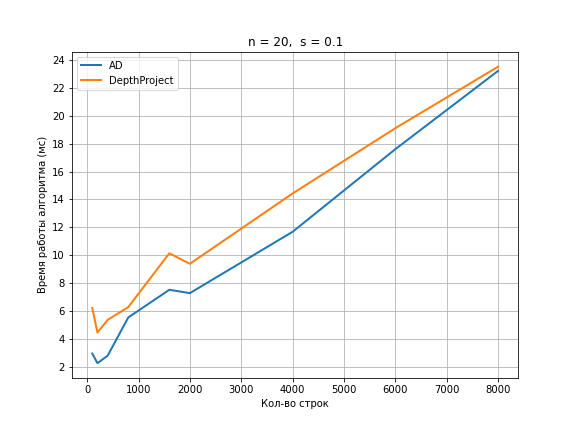
\includegraphics[scale=0.5]{r3p3.png}}
\caption{Зависимость времени работы от кол-ва строк}
\label{fig:image}
\end{figure}

Время работы двух алгоритмов асимптотически совпадает. Ниже представлен график отношения скоростей счёта:

\begin{figure}[H]
\center{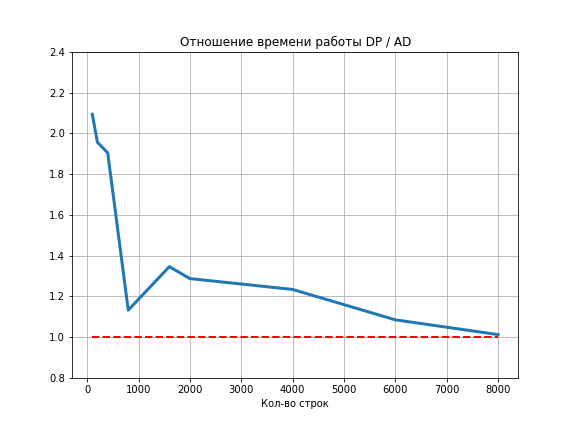
\includegraphics[scale=0.5]{r3p4.png}}
\caption{Отношение времени работы DepthProject и AD}
\label{fig:image}
\end{figure}

\section{Вывод}

Алгоритмы AD и DepthProject совершают одинаковое число шагов, имеют схожую сложность шага и выводят наборы в алфавитном порядке. Основное отличие заключается в том, что AD выполняется последовательно и использует меньше вычислительных ресурсов, в то время как DepthProject работает рекурсивно и строит полное дерево решений.

\section{Дополнение}

\subsection{Удаление нечастых столбцов}

Пусть дана бинарная матрица $T \in B^{m \times n}$, $B = \{0, 1\}$ и минимальная поддержка $s \in [0, 1]$. Мы можем удалить все столбцы матрицы T, имеющие меньше $m \cdot s$ единиц, ведь они не войдут ни в один частый набор. Назовём такие столбцы нечастыми.

Обозначим среднее количество нечастых столбцов за $Y$. Пусть матрица $T$ является случайной и берётся из равномерного распределения. Ясно, что при малых $s$ нечастых столбцов почти не будет, а при $s \approx 0.5$ и $s > 0.5$ такие столбцы почти наверное найдутся. Посчитаем, при каких $s, m, n$ среднее количество таких столбцов отлично от нуля.

Элементы матрицы $T$ имеют распределение Бернулли с $p = 0.5$. Следовательно, распределение единиц в отдельно взятом столбце представляет собой биномиальное распределение. Обозначим кол-во единиц в столбце за $k$, тогда \newline

$P(k = i) = C_m^i \cdot (\frac{1}{2})^i \cdot (\frac{1}{2})^{m-i} = \frac{1}{2^m} \cdot C_m^i$. \newline

Тогда несложно посчитать вероятность того, что столбец нечастый: \newline

$P(k < s) = \sum_{i = 0}^{s-1} P(k = i) = \frac{1}{2^m} \cdot \sum_{i = 0}^{s-1}C_m^i$ \newline

Чтобы найти среднее количество нечастых столбцов умножим полученную вероятность на $n$. Окончательно получим:\newline

$Y = \frac{n}{2^m} \cdot \sum_{i = 0}^{s-1}C_m^i$\newline

Можно показать, что $Y > 1$ начиная с $s > 0.4 \cdot m$ (примерно). Итак, если минимальная поддержка $s > 0.4$, то есть смысл перед поиском частых наборов удалить нечастые столбцы.

\end{document}